\documentclass[a4paper,12pt]{article}
\usepackage[a4paper,top=1.0cm, bottom=1.5cm, left=1.2cm, right=1.2cm]{geometry}

\usepackage[T2A]{fontenc}			
\usepackage[utf8]{inputenc}		
\usepackage[english,russian]{babel}	
\usepackage{amsmath,amsfonts,amssymb,amsthm,mathtools} 
\usepackage{wasysym}
\usepackage{graphicx}
\usepackage{wrapfig}
\usepackage{hyperref}
\usepackage{subcaption}
\DeclareGraphicsExtensions{.pdf, .png, .jpg}
\graphicspath{{}}

\begin{document}
	
	\section{Limitations}
	The task is to learn LLM to add 2 random numbers of longest lengths possible. The limitations of model considered:
		\begin{itemize}
			\item Only integer numbers
			\item Only positive numbers
		\end{itemize}
		The first limitation is not really a limitation -- a sum of decimal point numbers can be easily calculated in 2 steps with a model that can add integers by spliting numbers by decimal point and calculating partial sums separately. I did not implement that, because this seems like not the point of the task.\\
		The overcome the second one, the model should also learn how to subtract numbers or another model learned to subtract is needed, than simple preprocessing reduces the sum of any sign numbers to a single subtraction or addition. Not implemented because it would be a simple code repetition and twice of a training time.
	
	\section{Approaches}
		\subsection{Full model fine-tuning}
			One of the largest model that fits my local GPU without additional precision reduction is base version (220m parameters) of \href{https://arxiv.org/abs/1910.10683}{T5} from \href{https://huggingface.co/}{Hugging Face}. First approach is to take it's pre-trained version and learn on random generated numbers. As it is a language model, during initial learning steps I add some random text prompts like <<Calculate the following ... >>, <<The sum of .. and .. is >> etc. to supposedly enhance model ability to understand the task. After some training remove the prompts as the model is small enough for proper training and continue with <<a + b = >> input format.
		
		\subsection{LoRA}
			The second approach is to train just a low rank adaptors (\href{https://arxiv.org/abs/2106.09685}{LoRA}) for a bigger model (large version of T5). That requires less training time to achieve convergence and for much more difficult tasks results in impressive tuning profit on comparably weak hardware. Although it is a widely used well-performing approach, I doubt that it could beat fine tuning of a relatively small model in such a simple task. I use get\_peft\_model() function with LoraConfig from \href{https://huggingface.co/docs/peft/main/en/package_reference/tuners#peft.PromptEncoderConfig}{hugging face peft package} to apply LoRA on T5-large. 
		
		\subsection{RNN aka cheatcode for calculation}
			I'm not quite sure if a simple RNN model trained only with numbers' and EOS tokens can be called language model, but it is surely a quite effective approach as it can work very similar to manual calculation. (And, technically, the same architecture with larger tokenizer can be used as LM). Let's make a unique token for each digit pair and add a special one for the end of the input, than reverse both numbers, pad the shorter one with zeros, tokenize each digit pair, add EOS token and feed this sequence to the network. I expect this to get close to 1.0 accuracy on numbers of any lengths treating them as strings -- natural language sequences, even though it cannot process the language itself. 		
			
	\section{Training}
		\begin{itemize}
			\item[GPU:] 1660ti 6GB
			\item[Optimizer:] \href{https://arxiv.org/abs/1804.04235}{Adafactor} from \href{https://huggingface.co/docs/transformers/main_classes/optimizer_schedules}{transformers} package
			\item[Dataset:] Random generated numbers from of various length (check dataset\_generator.py)
			\item[Metrics:] Accuracy and average per-digit accuracy. The latter taken to check if the model miscalculated couple of digit in a long number or performed completely wrong
			\item[Loss:] In-built cross-entropy loss for pre-trained model and one from \href{https://pytorch.org/docs/stable/nn.functional.html}{torch.nn.functional} for RNN
		\end{itemize}
		The training starts with 100000 random number pairs dataset fed into the network, than restarts if necessary until the loss stop lowering. I use default adafactor options so it controls the learning rate automatically. Every 100 iterations the loss graph is displayed to be able to see what is going on. \\
		For the fine-tuning, learning starts with lengths of input number being up to 30 digits and than continues on a longer ones up to 100. Attempts to get meaningful results with longer numbers failed.\\
		For the LoRA  I stopped at 30 digits as it was unable to provide valid results even with such short numbers.\\
		RNN was originally trained on 1-200 digits random numbers, though it should be able to handle numbers of any length with the same results due to the architecture.

	\section{Inference and testing}
		For the inference, each model has the .generate(self, a, b) method that takes 2 int or str numbers and provide the output str in decoded form, that hopefully consists of only numbers. Lengths is unlimited, but all models apart from RNN have poor quality on longer numbers than ones they were trained on. Everything to run a model can be found in main.ipynb file, .py files provide functions and classes used for training and inference.\\
		I evaluated each model on several datasets of 1000 random number pairs of different lengths ranges and here is the results: 
		
		\begin{figure}[h!]
			\begin{subfigure}[h]{0.5\linewidth}
				\centering
				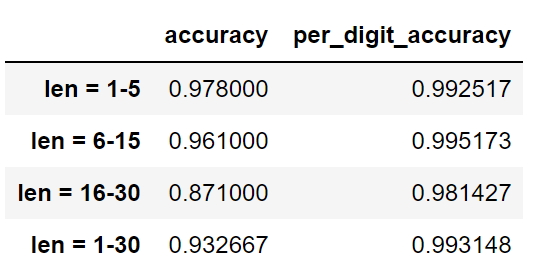
\includegraphics[scale=0.5]{figures/t5-base_metrics_30.png}
				\caption{FT for $\leqslant 30$ digits}
			\end{subfigure}
			\hfill
			\begin{subfigure}[h]{0.5\linewidth}
				\centering
				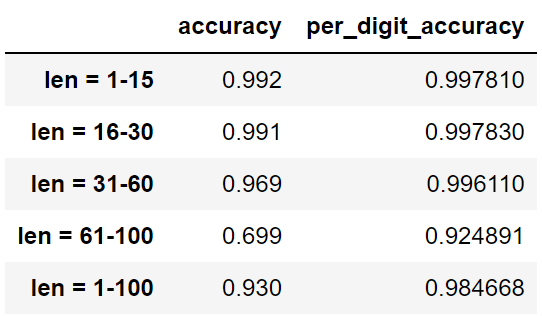
\includegraphics[scale=0.5]{figures/t5-base_metrics_100.png}
				\caption{FT for $\leqslant 100$ digits}
			\end{subfigure}
			\hfill
			\begin{subfigure}[h]{0.5\linewidth}
				\centering
				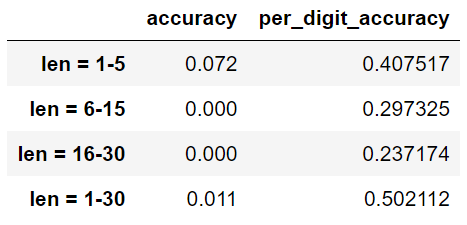
\includegraphics[scale=0.5]{figures/t5-large_lora_metrics_30.png}
				\caption{LoRA for $\leqslant 30$ digits}
			\end{subfigure}
		\begin{subfigure}[h]{0.5\linewidth}
			\centering
			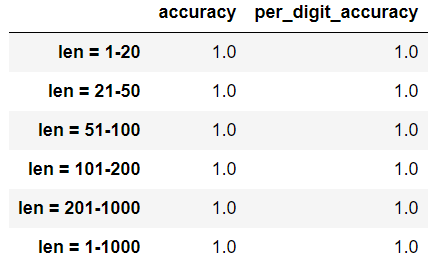
\includegraphics[scale=0.5]{figures/RNN_metrics.png}
			\caption{RNN}
		\end{subfigure}
			\caption{Evaluation results}	
		\end{figure}
	
	As we can see, for such a simple task using advanced methods like LoRA is unreasonable, at least with relatively small models that fit average consumer grade GPU. As expected, recurrent network meets perfect quality on numbers of any lengths. Fine-tuning of T5-base transformer also provides quite good accuracy on numbers up to 60 digits. Remarkably, per-digit accuracy is much higher than accuracy in case the model significantly underperforms, thus we can assume that even though it fails to provide the correct answer, the mistakes are minor and model processes significant part of the number correctly.

\end{document}


